\documentclass[10pt]{article}
\usepackage[margin=0.78in]{geometry}
\usepackage{amsmath,graphicx,booktabs,url}
\title{Battery Storage Dispatch Scheduling for a Hybrid Solar-Wind Microgrid}
\author{rishav76dev}
\date{}
\begin{document}
\maketitle
\begin{abstract}
We evaluate forecast-informed adaptive-reserve model predictive control (MPC) for battery dispatch in a constructed islanded solar--wind microgrid. The chronologically frozen 2025 holdout contains 4,176 operational hours plus a common 24-hour terminal-inventory normalization. Greedy, tuned fixed-reserve, adaptive-reserve and envelope-matched scenario MPC all serve operational demand without shortfall in this base case. Adaptive MPC has a lower BLAST-Lite capacity-loss estimate than fixed reserve (1.2140\% versus 1.2360\%), but its weekly-block paired confidence interval includes zero and every primary ageing update falls below the model's fitted cycle-depth range. Direct operating measures show nearly equal throughput and equivalent full cycles for the matched methods, while adaptive control lowers time above 80\% state of charge relative to fixed reserve. Corrected simultaneous deficit-envelope coverage is 91.26\% overall but 70.39\% in February. These results document an operational trade-off and model limitations; they do not establish battery-life superiority or seasonal 95\% calibration.
\end{abstract}

\section{Objective and case}
The objective is to develop and evaluate a forecast-informed adaptive-reserve MPC framework for battery dispatch in an islanded hybrid solar--wind microgrid, and assess its operational reliability, battery operating stress and computational performance against established dispatch strategies under common physical constraints. We ask whether adaptive reserve offers a useful trade-off among these quantities. This paper reports the frozen experiment and does not select a different comparator from the 2025 results.

Demand is scaled Indian national hourly demand attributed to Mukherjee, Kalita and Kumar\cite{demand}; generation is a simplified conversion of Jaisalmer NASA POWER weather\cite{power}. The combination is a constructed reference case, not measurements from a village or independent site. A 2022 forecaster and 2023 synchronized residual library feed online calibration initialized in January--June 2024. Hardware and controller settings were selected on July--December 2024, then frozen before the January 1--June 24, 2025 holdout. PV and wind nameplates are 95.653 and 126.764 kW. The battery has 400 kWh rated capacity, 50 kW power, 10--90\% SOC bounds and 95\% one-way efficiencies.

\section{Dispatch and evaluation}
Every controller uses the same single-bus hourly balance,
\begin{equation}
P_{PV}+P_{wind}+P_b+P_{unserved}=P_{load}+P_{curtailed},
\end{equation}
with positive battery power on discharge. The greedy reference serves current demand with available renewable energy and battery energy. The fixed-reserve MPC uses a validation-tuned constant target. Adaptive-reserve MPC adds a calibrated upper bound on each contiguous future DC-deficit interval to a validation-selected buffer, with physical-full fallback when the request is infeasible. Scenario MPC receives the same envelope; it uses scenario-specific future recourse and is therefore an optimistic two-stage benchmark. Current measured demand is served whenever physically feasible. The primary comparator is a separately calibrated adaptive-reserve variant selected on validation modelled damage. It is retained even though it fails the test reliability margin.

Operational energy LPSP is EENS divided by operational demand. Reliability matching requires the paired upper EENS difference to stay within 0.01 percentage points of operational demand at both 24-hour and 168-hour circular-block bootstrap lengths, with equal terminal energy. The test uses 1,000 replicates at each length. A positive ageing-superiority statement additionally requires negative paired damage upper bounds at both lengths, a practically meaningful reduction and stability under model/condition sensitivity. No bootstrap replication increase is used to seek significance. The last 24 hours use one common recharge-only policy: battery discharge is disabled, and all controllers reach 360 kWh. The normalization day is excluded from operational EENS and included in all-hours EENS and ageing.

\section{Base-case results}
\begin{table}[ht]
\centering\small
\begin{tabular}{lrrrrr}
\toprule
Method & Op. EENS & All EENS & LoL hours & High-SOC hours & BLAST loss \\
 & kWh & kWh & h & $>80\%$ SOC & \% \\
\midrule
Greedy & 0 & 9.160 & 0 & 2058 & 1.2376 \\
Independent adaptive (preselected) & 12.308 & 21.468 & 2 & 1464 & 1.1934 \\
Fixed reserve & 0 & 9.160 & 0 & 2037 & 1.2360 \\
Adaptive reserve & 0 & 9.160 & 0 & 1755 & 1.2140 \\
Scenario + matched envelope & 0 & 9.160 & 0 & 1763 & 1.2148 \\
\bottomrule
\end{tabular}
\caption{Frozen 2025 holdout. The first 4,176 hours are operational; the common final 24 hours add 9.1599 kWh EENS for every method. All terminal inventories are 360 kWh. BLAST-Lite values are exploratory model estimates, not measured ageing.}
\end{table}

The preselected independent comparator sheds 12.308 kWh (0.0210\% operational LPSP), beyond the 5.8652 kWh matching allowance. Its lower modelled damage cannot support a matched-reliability benefit. Greedy, fixed reserve, adaptive reserve and envelope-matched scenario MPC have zero operational EENS, zero loss-of-load hours and equal terminal inventory. Their paired EENS upper differences are zero at both block lengths. Adaptive versus fixed reserve reduces modelled loss by 0.0220 percentage points (1.78\% relative); its 168-hour paired damage interval includes zero. Adaptive versus envelope-matched scenario MPC differs by only 0.0008 percentage points of modelled loss; its daily and weekly damage intervals both include zero. Thus no robust matched-reliability ageing superiority is established.

Direct battery-stress measures support a narrower interpretation. Greedy, fixed, adaptive and envelope-matched scenario controllers each have approximately 47,626 kWh operational DC throughput and 59.575 all-hours rainflow equivalent full cycles. Adaptive control has 1,755 of 4,176 operational hours above 80\% SOC, versus 2,037 for fixed reserve and 1,763 for scenario MPC. Its operational mean SOC is 0.7234, compared with 0.7477 and 0.7243 respectively. Rainflow depth distributions and the reproducible extraction script accompany the release. These measures describe operation; none is an observed capacity-loss measurement.

\section{Forecasts, uncertainty and computation}
The learned forecast has 5.299 kW pooled future-lead MAE and 10.127 kW RMSE, versus 4.591 kW MAE for weekly persistence; a comparable persistence RMSE was not released. Forecast superiority is therefore not claimed. Corrected simultaneous deficit-envelope coverage improves from 19.34\% raw to 91.26\% over the holdout, but it is 70.39\% in February and misses nominal 95\% overall. The monthly pattern appears in Fig.~\ref{fig:coverage}. For the adaptive method, the recorded reserve-infeasible fraction is 34.38\% of all hours; the same envelope makes scenario MPC's fraction equal. The independent variant records 25.81\%. At the end of each adaptive dispatch step, stored energy meets the recorded requested target in 34.87\% of operational hours. Reserve requests are capped at physical full storage when infeasible. Monthly envelope-width records were not preserved in the released summary, so coverage alone cannot establish sharpness.

\begin{figure}[ht]
\centering
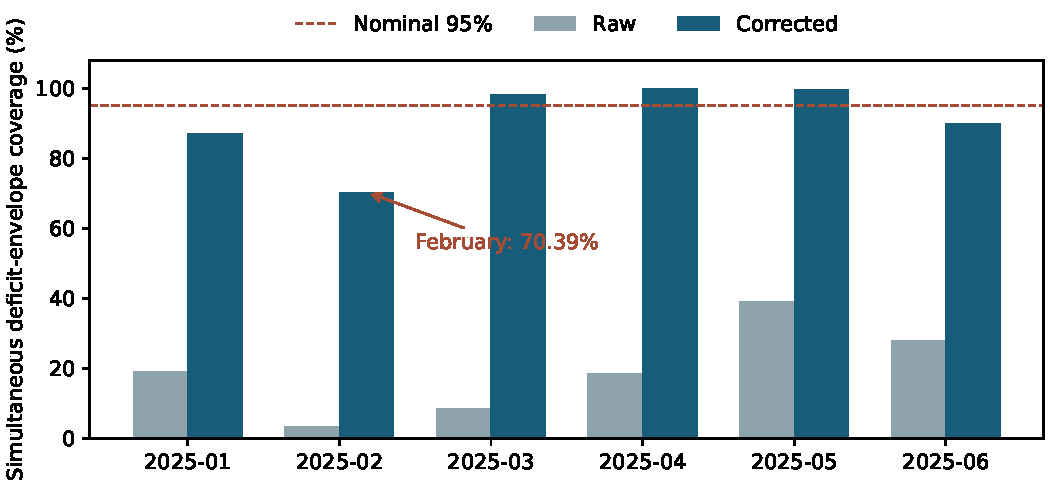
\includegraphics[width=.88\linewidth]{../docs/revision_evidence/monthly_coverage.pdf}
\caption{Raw and corrected simultaneous DC-deficit-envelope coverage by 2025 local month. February undercoverage is visible. June is partial.}\label{fig:coverage}
\end{figure}

Recorded controller-only p95 times are 7.64 ms for adaptive MPC and 250.74 ms for envelope-matched scenario MPC. Batched forecasting and shared scenario preparation were measured under a different scope, so these numbers are descriptive implementation timings rather than an end-to-end live latency comparison or an algorithmic speedup claim. A same-environment repeated benchmark is required before a computational-superiority claim.

\section{Ageing applicability and limitations}
The published BLAST-Lite LFP-Gr model is implemented with numerical checks against the pinned source\cite{blast}. At assumed 25$^\circ$C, all 175 primary adaptive daily windows fall below its fitted 80--100\% depth-of-discharge range. The 35$^\circ$C and 12/48-hour replays test calculation sensitivity, not empirical pack applicability. An independent published LFP cycle model by Wang et al.\cite{wang} includes 10\% cycle depth but starts at C/2 discharge; this system's maximum rated power is C/8. A second numerical ageing estimate would thus introduce a different extrapolation. We use throughput, equivalent full cycles, SOC exposure and cycle-depth distribution as primary battery-stress evidence and label BLAST-Lite estimates exploratory.

All four principal base-case controllers have zero operational EENS, limiting reliability discrimination. A renewable-shortage sensitivity requires a derating chosen on development data and consistent derating of actual PV/wind, forecasts and scenarios. The raw hourly source and frozen forecast/scenario arrays are not included in the committed review release, so that controller experiment is not reported here. The load proxy, simplified weather-to-generation conversion, single site, assumed battery temperature and lack of independent pack measurements further limit generalization. The contribution is a physically constrained adaptive-reserve dispatch comparison with explicit reliability, battery-stress and uncertainty-calibration diagnostics, not a claim that the proposed method dominates every baseline.

\bibliographystyle{plain}
\bibliography{references}
\end{document}
